\section{Design}
\label{s:gen}

\autoref{f:flow} shows \sys's workflow.  Given the LLVM intermediate
representation~(IR) compiled from source code, \sys generates a set
of constraints for each integer operation, and feed them into the
Boolector constraint solver for deciding satisfiability.

Specifically, \sys generates three types of constraints.
%
Given an integer operation, the error constraint is generated
directly from definition.
%
\sys also calculates the path constraint, the predicate satisfying
which the operation is reachable from the start of that function.
%
To further improve accuracy, \sys infers additional range information
of function parameters and structure fields across the call graph.
It also allows users to provide annotations as constraints.

\begin{figure}
\centering
\resizebox{\linewidth}{!}{
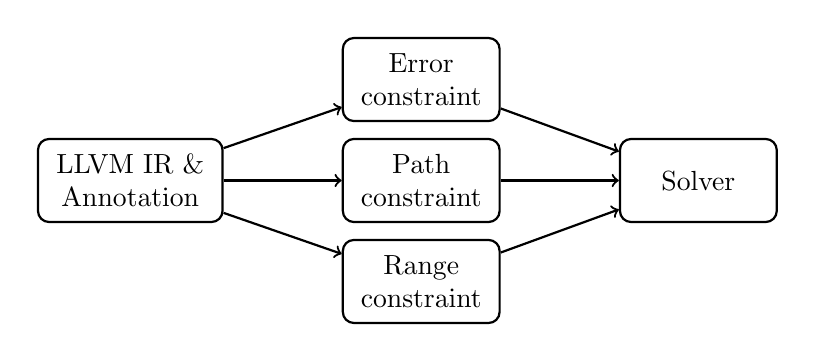
\begin{tikzpicture}[
	block/.style={
		rectangle, rounded corners,
		draw=black, thick,
		text width=5em, minimum height=3em, text centered
	},
	line/.style={draw, thick, ->},
	]
	\matrix[row sep=2mm, column sep=15mm] {
		& \node [block] (ec) {Error constraint}; & \\
		\node [block, text width=6em] (ir) {LLVM IR \& Annotation};
		& \node [block] (pc) {Path constraint};
		& \node [block] (sol) {Solver}; \\
		& \node [block] (rc) {Range constraint}; & \\
	};

	\path [line] (ir) -- (ec);
	\path [line] (ir) -- (pc);
	\path [line] (ir) -- (rc);
	\path [line] (ec) -- (sol);
	\path [line] (pc) -- (sol);
	\path [line] (rc) -- (sol);
\end{tikzpicture}

}
\caption{\sys's workflow.  It generates constraints from the LLVM
intermediate representation~(IR) and user annotations, and then feeds
the constraints to a solver for satisfiability testing.}
\label{f:flow}
\end{figure}

\subsection{Error Constraint Generation}
\label{s:gen:err}

For arithmetic and shift operations, it is straightforward to
generate their error constraints from their definitions shown in
\autoref{s:sema:constr}.  As for $n$-bit unsigned multiplication,
one may use a $2n$-bit binary multiplier (extending both integers
from $n$ to $2n$ bits first), which flags an overflow error if any
of the most significant $n$ bits of the product is
1~\cite{molnar:catchconv}.

Boolector provides highly optimized Boolean circuits for implementing
some of these error constraints.  Its overflow detection circuit,
for example, does not even need to compute the $2n$-bit product and
thus can be solved far more
efficiently~\cite[\chapterautorefname~3.5]{brummayer:phd}.  \sys
reuses these circuits for better performance.

\sys deals with the two conversion cases as follows.

To detect tautological comparisons, \sys derives a predicate from
each comparison.  If the predicate is trivially true or false
resulted from an integer conversion within that function, \sys
reports the conversion as an integer error.

For negative counts, it is easy to generate the error constraint
for a value $x$ that should be conceptually non-negative, that is,
$x <_s 0$; however, \sys needs to know them first.  \sys implements
a front-end plugin to recognize array indices.  \sys also requires
user-provided annotations on ``size'' function parameters.  As for
the Linux kernel, we annotate parameters in functions like \cc{memcpy},
\cc{copy_from_user}, and \cc{sock_alloc_send_skb}.

\subsection{Path Constraint Generation}

We use \autoref{f:ax25-sign} as an example to illustrate how \sys
generates path constraints.  The control flow of the code is shown
in \autoref{f:cfg}, where there are two sanity checks on \cc{optlen}
before it reaches \cc{copy_from_user}.  For clarification purpose
\cc{optlen} is numbered every time it is assigned a new
value~\cite[\chapterautorefname~8.11]{whale}.  Our goal is to
evaluate the path constraint for the call to \cc{copy_from_user}.

The basic algorithm works as follows.  Since there is no loop, the
path constraint of the call to \cc{copy_from_user} is simply the
logical OR of the constraint from each of its predecessors, namely
\textsc{If-True} and \textsc{If-False}.  For each predecessor, the
constraint is a logical AND of three parts: the branching condition,
possible assignment(s) in the predecessor, and the path constraint
of that predecessor.  Here both \textsc{If-True} and \textsc{If-False}
unconditionally jump to \cc{copy_from_user}, so their branching
conditions are simply true, which can be ignored.  Now we have the
path constraint as follows:
\newcommand{\optlen}{{\small \texttt{optlen}}}
\newcommand{\pc}{\textrm{PathConstraint}}
%
\begin{align*}
& ((\optlen_1 = 16) \land \pc(\textsc{If-True})) \\
\lor & ((\optlen_1 = \optlen_0) \land \pc(\textsc{If-False})).
\end{align*}

Recursively apply the algorithm to \textsc{If-True} and \textsc{If-False},
and we can get the fully expanded result:
%
\begin{align*}
& ((\optlen_1 = 16) \land (\optlen_0 >_s 16)
    \land \neg(\optlen_0 <_u 4)) \\
\lor & ((\optlen_1 = \optlen_0) \land \neg(\optlen_0 >_s 16) \\
     & \; \land \neg(\optlen_0 <_u 4)).
\end{align*}

One can feed the logical AND of the path constraint and the error
constraint (i.e., $\cc{optlen}_1 <_s 0$) into the solver, which
will reply with an error example, e.g., $\cc{optlen}_0 = -1$.

\begin{figure}
\centering
\resizebox{\linewidth}{!}{
\begin{tikzpicture}[
	->, >=stealth', node distance=2.4cm, semithick,
	block/.style={
		rectangle, draw, rounded corners,
		text centered, minimum width=3em, minimum height=2.5em
	},
	]

	\node [block] (entry) {\begin{tabular}{l}
		\cc{char devname[IFNAMSIZ];} \\
		$\cc{if}\ (\cc{optlen}_0 < \cc{sizeof}(\cc{int}))$
	\end{tabular}};

	\node [block, below of=entry] (if) {\begin{tabular}{l}
		$\cc{if}\ (\cc{optlen}_0 > \cc{IFNAMSIZ})$
	\end{tabular}};

	\node [block, below of=if, xshift=-2.4cm] (true) {\begin{tabular}{l}
		\textsc{If-True:} \\
		$\cc{optlen}_1 = \cc{IFNAMSIZ;}$
	\end{tabular}};

	\node [block, below of=if, xshift=2.4cm] (false) {\begin{tabular}{l}
		\textsc{If-False:} \\
		$\cc{optlen}_1 = \cc{optlen}_0\cc{;}$
	\end{tabular}};

	\node [block, below of=true, xshift=2.4cm] (copy) {\begin{tabular}{l}
		$\cc{copy_from_user}(\cc{devname}, \cc{optval}, \cc{optlen}_1)\cc{;}$ \\
		...
	\end{tabular}};

	\node [block, below of=copy, xshift=-3cm, minimum width=10em] (exit) { EXIT };

	\path
		(entry) edge node[anchor=west]{$\neg(\cc{optlen}_0 <_u 4)$} (if)
		(entry) edge[bend right=65] (exit)
		(if) edge node[anchor=east]{$\cc{optlen}_0 >_s 16$} (true)
		(if) edge node[anchor=west]{$\neg(\cc{optlen}_0 >_s 16)$} (false)
		(true) edge node[anchor=east]{$\cc{optlen}_1 = 16$\, } (copy)
		(false) edge node[anchor=west]{$\cc{optlen}_1 = \cc{optlen}_0$} (copy)
		(copy) edge (exit)
		;
\end{tikzpicture}

}
\caption{The control flow of the code snippet in \autoref{f:ax25-sign}.}
\label{f:cfg}
\end{figure}

For complex programs that contain loops, \sys handles them using
the standard unrolling technique~\cite{xie:saturn}.  The path
constraint generation algorithm unrolls each loop once and ignores
branching edges that jump back in the control flow, aka back edges.
The complete algorithm is listed in \autoref{f:path-cstr}.

\begin{figure}
\begin{algorithmic}
\Function{PathConstraint}{$\mathit{blk}$}
\State $g \gets \textbf{false}$
\ForAll{$\mathit{pred} \in \mathit{blk}$'s predecessors(s)}
\State $e \gets (\mathit{pred},\mathit{blk})$
\If{$e$ is not a back edge}
	\State $\mathit{br} \gets e$'s branching condition
	\State $\mathit{as} \gets \bigwedge_i(x_i = y_i)$ for all assignments along $e$
	\State $g \gets g \lor (\Call{PathConstraint}{\mathit{pred}} \land \mathit{br} \land \mathit{as})$
\EndIf
\EndFor
\State \Return{$g$}
\EndFunction
\end{algorithmic}

\caption{Algorithm for path constraint generation.}
\label{f:path-cstr}
\end{figure}

\subsection{Range Constraint Generation}

\sys generates range constraints for function parameters
and structure fields.

%handle sysctl interface.


\subsection{Optimizations}

\paragraph{In-loop constraint.}
\sys tries to move constraints within a loop to the outside scope
so as to generate more constraints.  Consider the following loop.
\begin{Verbatim}[commandchars=\\\{\},codes={\catcode`\$=3\catcode`\^=7\catcode`\_=8}]
\PY{k}{for} \PY{p}{(}\PY{n}{i} \PY{o}{=} \PY{l+m+mi}{0}\PY{p}{;} \PY{n}{i} \PY{o}{\PYZlt{}} \PY{n}{n}\PY{p}{;} \PY{o}{+}\PY{o}{+}\PY{n}{i}\PY{p}{)}
    \PY{n}{a}\PY{p}{[}\PY{n}{i}\PY{p}{]} \PY{o}{=} \PY{p}{.}\PY{p}{.}\PY{p}{.}\PY{p}{;}
\end{Verbatim}

\sys will generate an error constraint $i <_s 0$ since $i$ is used
as an array index.  As $i$ also is a loop variable, \sys will move
the constraint out of the loop and rewrite it as $n <_s 0$, by
substituting the loop variable $i$ with its exit value $n$.

\paragraph{Pointer arithmetic.}
\sys represents each pointer or memory address as a symbolic
expression~\cite{engelen:symbolic}, and tries to simplify it if
possible.  A pointer expression that \sys fails to simplify will
be considered as a black-box integer, which can be any value within
its range.  Consider the code snippet below.
%
\begin{Verbatim}[commandchars=\\\{\},codes={\catcode`\$=3\catcode`\^=7\catcode`\_=8}]
\PY{k}{struct} \PY{n}{pid\PYZus{}namespace} \PY{p}{\PYZob{}}
    \PY{k+kt}{int} \PY{n}{kref}\PY{p}{;}
    \PY{k}{struct} \PY{n}{pidmap} \PY{n}{pidmap}\PY{p}{[}\PY{n}{PIDMAP\PYZus{}ENTRIES}\PY{p}{]}\PY{p}{;}
    \PY{p}{.}\PY{p}{.}\PY{p}{.}
\PY{p}{\PYZcb{}}\PY{p}{;}
\PY{k}{struct} \PY{n}{pid\PYZus{}namespace} \PY{o}{*}\PY{n}{pid\PYZus{}ns} \PY{o}{=} \PY{p}{.}\PY{p}{.}\PY{p}{.}\PY{p}{;}
\PY{k+kt}{unsigned} \PY{k+kt}{int} \PY{n}{last} \PY{o}{=} \PY{p}{.}\PY{p}{.}\PY{p}{.}\PY{p}{;}
\PY{k}{struct} \PY{n}{pidmap} \PY{o}{*}\PY{n}{map} \PY{o}{=}
    \PY{o}{&}\PY{n}{pid\PYZus{}ns}\PY{o}{-}\PY{o}{>}\PY{n}{pidmap}\PY{p}{[}\PY{p}{(}\PY{n}{last} \PY{o}{+} \PY{l+m+mi}{1}\PY{p}{)}\PY{o}{/}\PY{n}{BITS\PYZus{}PER\PYZus{}PAGE}\PY{p}{]}\PY{p}{;}
\PY{k+kt}{int} \PY{n}{off} \PY{o}{=} \PY{n}{map} \PY{o}{-} \PY{n}{pid\PYZus{}ns}\PY{o}{-}\PY{o}{>}\PY{n}{pidmap}\PY{p}{;}
\end{Verbatim}

%
The offset of \cc{pidmap} in the structure \cc{pid_namespace} is 4
bytes, i.e., the size of \cc{kref}, thus \sys represents the address
\cc{pid_ns->pidmap} as $\cc{pid_ns} + 4$.  Here \cc{pid_ns} is
considered as a black box since no further information is available.

In addition, assuming the size of each element of \cc{pidmap} is 8
bytes, \sys represents the address \cc{\&pid_ns->pidmap[i]} as
$\cc{pid_ns} + 4 + i \times 8$; in this example we have $i =
(\cc{last} + 1) /_u \cc{BITS_PER_PAGE}$.  Thus, the value of \cc{off},
the subtraction of the two pointers, is reduced to $(\cc{pid_ns} +
4 + i \times 8) - (\cc{pid_ns} + 4) = i \times 8$.

\paragraph{Value equality testing.}
How to determine the values from two load instructions
are the same? Load hoisting, unsound aliasing rules.

%\autoref{f:hoist} shows in the hoisting algorithm.

aliasing assumption~\cite{livshits:ipssa}.
\sys assumes that a pointer passed as a function parameter or a
global variable points is distinct from any other memory location.


\if 0
\begin{figure}
\begin{algorithmic}
\footnotesize
\Procedure{Hoist}{$I$}\Comment{$I$ is a load instruction}
\State $\mathit{loc} \gets I$'s memory location to load from
\Loop
\If{\textbf{not} \Call{HoistInBlock}{$I$, $\mathit{loc}$}}
	\State \Return
\EndIf
\State $\mathit{blk} \gets$ \Call{ChooseTargetBlock}{$I$, $\mathit{loc}$}
\If{$\mathit{blk} = \textbf{nil}$}
	\State \Return
\EndIf
\State Move $I$ to the end of $blk$
\EndLoop
\EndProcedure
\\
\Function{HoistInBlock}{$I$, $\mathit{loc}$}
\Loop
\State $\mathit{prev} \gets I$'s previous instruction in current block
\If{$\mathit{prev} = \textbf{nil}$}
	\Comment{Moved to beginning of the block?}
	\State \Return \textbf{true}
\EndIf
\If{$\mathit{prev}$ may modify $\mathit{loc}$ \textbf{or} \\
\hspace{3.6em} \textbf{not} $\mathit{loc}$ dominates $\mathit{prev}$}
	\State \Return \textbf{false}
\EndIf
\State Move $I$ before $\mathit{prev}$
\EndLoop
\EndFunction
\\
\Function{ChooseTargetBlock}{$I$, $\mathit{loc}$}
\State $\mathit{blk} \gets I$'s block
\State $\mathit{anc} \gets$ the common ancestor of $\mathit{blk}$'s predecessor(s)
\If{$\mathit{anc} = \mathit{blk}$ \textbf{or} \textbf{not} $\mathit{loc}$ dominates $\mathit{anc}$}
	\State \Return \textbf{nil}
\EndIf
\State $\mathit{blkset} \gets \{\mathit{anc}\}$
\If{\Call{CanBlocksModify}{$\mathit{loc}$, $blk$, $\mathit{blkset}$}}
	\State \Return \textbf{nil}
\EndIf
\State \Return $\mathit{anc}$
\EndFunction
\\
\Function{CanBlocksModify}{$\mathit{loc}$, $\mathit{blk}$, $\mathit{blkset}$}
\ForAll{$b \in \mathit{blk}$'s predecessor(s)}
	\If{$b \notin \mathit{blkset}$}
		\State $\mathit{blkset} \gets \mathit{blkset} \cup \{b\}$
		\ForAll{$\mathit{instr} \in b$}
			\Comment{Can $b$ modify $\mathit{loc}$?}
			\If{$\mathit{instr}$ may modify $\mathit{loc}$}
				\State \Return \textbf{true}
			\EndIf
		\EndFor
		\If{\Call{CanBlocksModify}{$\mathit{loc}$, $b$, $\mathit{blkset}$}}
			\State \Return \textbf{true}
		\EndIf
	\EndIf
\EndFor
\State \Return \textbf{false}
\EndFunction

\end{algorithmic}

\caption{The hoisting algorithm to move a load instruction to the
earliest possible point within a function.  It repeats the two
phases: first try to move the instruction to the beginning of its
basic block; if successful, try to move it into the common ancestor
of the block's predecessors.}
\label{f:hoist}
\end{figure}
\fi

\paragraph{Error-before-check.}
An integer error check may come after the overflowed computation,
but before any use of the result.  In that case, the overflowed
computation is benign.  Below is such an example.  Even the
multiplication $x \times_u y$ overflows, the product \cc{size} is
not used before the check.
\begin{Verbatim}[commandchars=\\\{\},codes={\catcode`\$=3\catcode`\^=7\catcode`\_=8}]
\PY{k+kt}{unsigned} \PY{n}{size} \PY{o}{=} \PY{n}{x} \PY{o}{*} \PY{n}{y}\PY{p}{;}
\PY{k}{if} \PY{p}{(}\PY{n}{x} \PY{o}{\PYZgt{}} \PY{n}{UINT\PYZus{}MAX} \PY{o}{/} \PY{n}{y}\PY{p}{)}
    \PY{k}{return} \PY{o}{-}\PY{l+m+mi}{1}\PY{p}{;}
\PY{p}{.}\PY{p}{.}\PY{p}{.} \PY{o}{=} \PY{n}{malloc}\PY{p}{(}\PY{n}{size}\PY{p}{)}\PY{p}{;}
\end{Verbatim}


To avoid warning against such cases, \sys invokes LLVM to push every
integer operation down to the latest possible point along the control
flow, so that the result is computed only when it is needed.  The
detail of the algorithm is omitted since it is similar to load
hoisting, except that it runs towards the opposite direction, and
does not need to consider memory loads and stores.

In the above example, \sys will move the integer operation $x
\times_u y$ down to right after the \cc{if} branch and before the
\cc{malloc} call, where its result \cc{size} is first used.

\paragraph{Error checking idiom.}

We notice that when generating path constraints some integer
operations like division would significantly slow down the constraint
solver~\cite{brummayer:perf}.  Many of such cases are used in integer
error checks like $N /_u x > y$, where $N$ is a constant and $x,
y$ are $n$-bit integers.  \sys recognizes such an integer error
checking idiom and rewrites it to avoid the division operation, as
follows.

In general, \sys first zero-extends $x$ and $y$ from $n$ to $2n$
bits, as $x_{2n}$ and $y_{2n}$, respectively, and rewrites the check
as multiplication $x_{2n} \times_u y_{2n} <_u N$.  If $N$ is a
special constant, such as $\uintmax(n)$ or $2^n-1$, \sys rewrites
the check with the multiplication overflow detection circuit (see
\autoref{s:gen:err}).

\autoref{f:udiv} shows a microbenchmark that measures the solving
time of the three checking forms of 32- and 64-bit integers,
respectively.  Each test is repeated 1000 times.  For a single
unsigned division operation this optimization can achieve up to
2.5$\times$ speedup.

\begin{figure}
\centering
\begin{tabular}{lr@{$\pm$}lr@{$\pm$}l} \toprule
Expression & \multicolumn{2}{c}{$n = 32$} & \multicolumn{2}{c}{$n = 64$} \\ \midrule
$\uintmax(n) /_u x > y$
& 10.02 & 0.03 & 43.93 & 0.22 \\
$x_{2n} \times_{u} y_{2n} > \uintmax(n)$
&  7.43 & 0.01 & 35.01 & 0.13 \\
$\umulo(x, y)$
&  4.36 & 0.13 & 17.25 & 0.40 \\
\bottomrule
\end{tabular}

\caption{Solving time of $\uintmax(n) /_u x > y$ and two variant
forms: $2n$-bit multiplication and the multiplication overflow
detection circuit, measured in milliseconds.}
\label{f:udiv}
\end{figure}

\subsection{Limitations}

We discuss what integer errors \sys could miss, i.e., false negatives.

\sys only understands C-language code; it will cannot detect integer
errors written in assembly language.

\sys cannot scan code that is not enabled for compilation in current
configuration or architecture.  One may enable as many modules as
possible for compilation or try different combinations for better
code coverage.

As discussed in \autoref{s:sema:def}, \sys's default semantics may
not apply to some architectures like PowerPC and will miss bugs
specific to those architectures.

\sys analyzes loops by unrolling them once, so it will miss integer
errors caused by looping, for example, an addition overflow in an
accumulation.

\sys's alias assumption is unsound, and thus it will miss bugs
caused by the assumption.

Finally, if the solver times out, \sys will miss the possible integer
error corresponding to the queried constraint.
